\section{Aim of the Study}\label{aim of study}

This section explains why the depthmap enhancement is needed, and how it would help the aquaculture industry. There is also an explanation of the challenges met by working with the Raytrix camera and the depthmap images.

\subsection{Scope}

The goal of this project is to help SEALAB on their way of making a complete camera system ready for underwater use for the aquaculture industry. SEALABs complete system should be able to detect the fish and classify it, measure the volume of the fish and detect salmon lice.
This projects focus is to better the depthmap images taken by the Raytrix camera so that the volume measurement becomes more accurate. Under the right light conditions and at some certain distance, this individual system should be able to measure the volume of an object underwater. The task is aimed towards fish, especially salmon, as this system would mostly benefit the salmon breeding industry.
The aquaculture breeding industry is currently selling their fish without any knowledge on how much they actually got. With a complete camera system in place in every underwater cage, an estimate of the total volume of fish can be made, salmon lice can be discovered earlier, and the companies can save huge amounts of money. 

The aim of this study is for the volume estimation of salmon to become more accurate. For this to happen, particles and unnecessary data needs to be removed and be replaced by relevant data. The depthmap computed by the Raytrix camera normally looks like the one in figure \ref{fig:depthmap82}, and it is seen from this image that there are holes in the fish, parts of the fish's belly and head is missing, and there are particles in front of the fish. This gives large opportunities for improvement, but also some challenges that need to be worked out.

\begin{figure}[H]
    \centering
    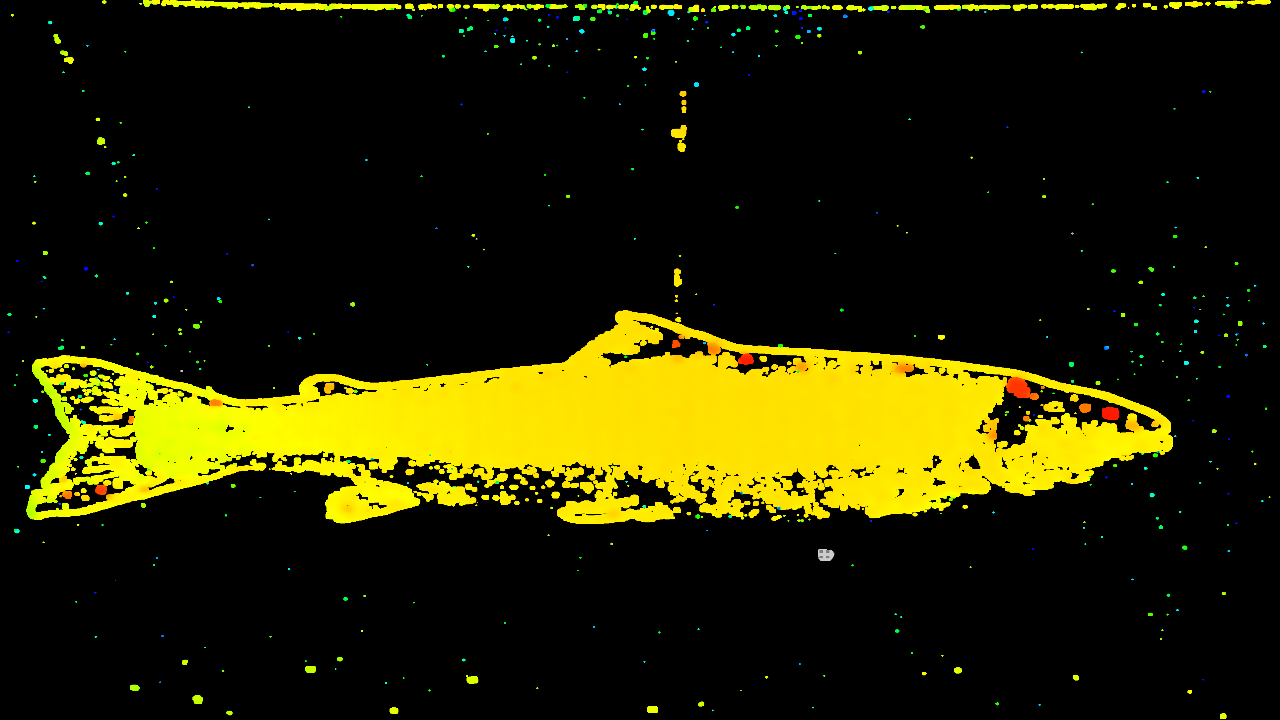
\includegraphics[width=.7\linewidth]{images/aim_of_study/depthmap82}
    \caption{Depthmap image of salmon}
    \label{fig:depthmap82}
\end{figure}


\subsection{Challenges}

The volume measurement is depending on the depth information stored in the depthmap image. For this measurement to be accurate, the data in the depthmap image must be more complete. Holes in the fish must be filled in while the shape of the fish remains.

A MATLAB 3D plot shows how bad the actual depth information is (see figure \ref{fig:matlab3D}). The particles make for large disturbances and the holes in the fish make for even bigger ones. The parts of the salmon that make for the largest depthmap errors is the belly, the fins and its head. The belly is white and the color is too close the the background color in the test facility. The head and fins are very black, and it could be a problem to the Raytrix that it is too black, and therefore makes it hard to see differences in each micro lens.

\begin{figure}[H]
    \centering
    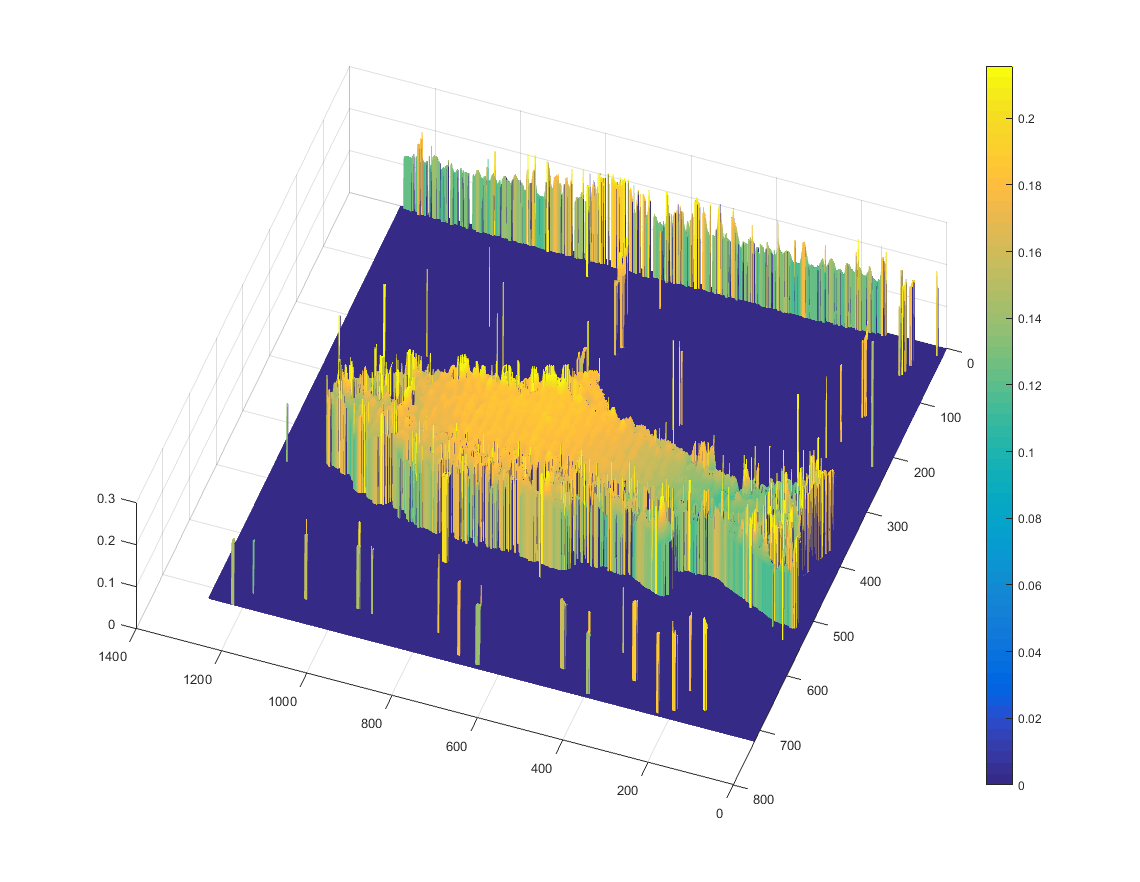
\includegraphics[width=.7\linewidth]{images/aim_of_study/original_3D_82}
    \caption{3D plot of depthmap}
    \label{fig:matlab3D}
\end{figure}

Even though there are many errors, it should be possible using the data from the depthmap image, enhance it and get a smooth surface of the fish, and thereby get a successful volume measurement. That is what the following sections in this report hope to show using the theory provided in section \ref{overview}.
